\documentclass[11pt,a4paper]{article}
\usepackage[hyperref]{acl2019}
\usepackage{times}
\usepackage{graphicx}
\usepackage{latexsym}

\usepackage{url}

% \aclfinalcopy % Uncomment this line for the final submission
%\def\aclpaperid{***} %  Enter the acl Paper ID here

\newcommand\BibTeX{B\textsc{ib}\TeX}

\title{BECON: \textbf{B}ERT with \textbf{E}vidence from \textbf{CON}ceptNet for Common Sense Question Answering}

\author{Shuailong Liang\textsuperscript{1}, Yue Zhang\textsuperscript{2}\\
    \textsuperscript{1}Singapore University of Technology and Design, Singapore\\
    \textsuperscript{2}School of Engineering, Westlake University, China\\
    {\tt shuailong\_liang@mymail.sutd.edu.sg}\\
    {\tt zhangyue@westlake.edu.cn}
}

\date{}

\begin{document}
\maketitle
\section*{Abstract}

CommonsenseQA~\cite{talmor2018commonsenseqa} is created based on knowledge graphs on ConceptNet ~\cite{speer2017conceptnet}. Solving the task requires the model to have common sense or world knowledge like humans. Current LM-pretrained model such as BERT~\cite{devlin2018bert} achieves state-of-the-art performance on the CQA dataset, which implies that language models trained on very large corpus may learn some sort of common sense knowledge implicitly. On the other hand, with the availability of the large knowledge graph such as ConceptNet, which contains explicit common sense knowledge, we would like to investigate how to use the explicit form of common sense knowledge as complementary to BERT which has implicit common sense knowledge.

For CommonsenseQA task, a question and five candidate answers are given, and one of the five answers is correct. The candidate answers usually consist of one or two words, forming a \textit{concept}. According to ~\cite{talmor2018commonsenseqa}, the best performing baseline model is the BERT-large model finetuned with CQA dataset. Our model is built based on BERT-large model, but also utilizes additional pieces of evidence from ConceptNet, which provides useful information to answer the question.

Concretely, to use the knowledge in Conceptnet, we first query each candidate answer in ConceptNet to get a list of evidence sentences which may be helpful to answer the question. In order to reduce the noise, we use pretrained BERT with Next-Sentence-Prediction head (BERT-NSP) to rank the evidence sentences and select the top-scored one. An example of the evidence sentences is shown in Figure~\ref{figure:introdemo}. We believe that BERT-NSP is helpful to rank the relevancy of the question and the evidence sentence. As in \cite{talmor2018commonsenseqa}, each question-answer pair is linearized into a delimiter-separated sequence (i.e., "{\tt[CLS]} If ... ? {\tt [SEP]} bedroom {{\tt [SEP]}") and the hidden vector over the {\tt [CLS]} token are used as representation of the choice. For our BECON model, we further concatenate the evidence sentence (i.e., "{\tt [CLS]} If ... ? {\tt [SEP]} bedroom {\tt [SEP]} bedroom is a place for sleeping {\tt [SEP]}"), which may help the model make better decisions.

\begin{figure}[t]
    \centering
    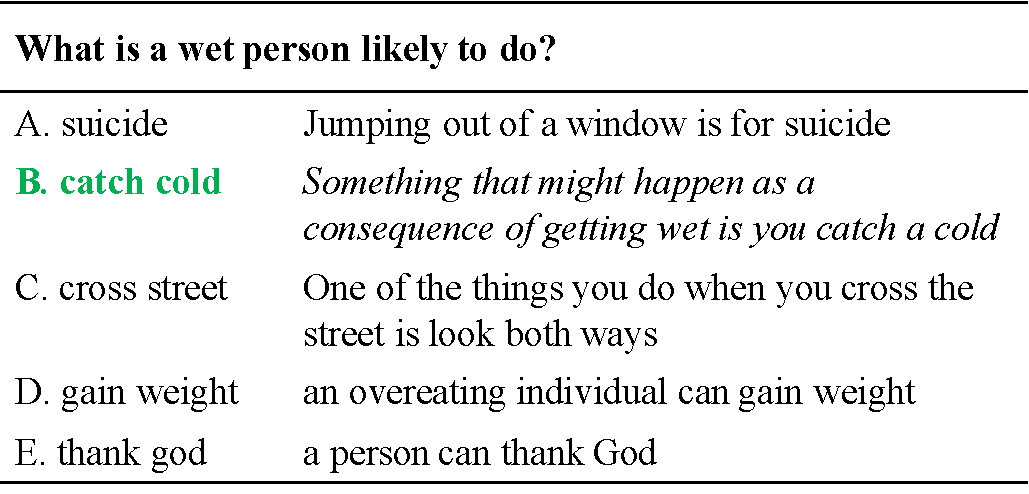
\includegraphics[width=\columnwidth]{figure}
    \caption{A question from CommonsenseQA dataset and its 5 candidate answers with their corresponding top-ranked evidences. The correct answer are in {\bf bold}/green, and the evidence corresponding to the correct answer is it {\it italic}.}
    \label{figure:introdemo}
\end{figure}

\begin{table}[t]
    \centering
    \small
    \begin{tabular}{l c}
    \hline
    {\bf Model}  & {\bf test F1 } \\
    \hline\hline
    BERT-large~\cite{talmor2018commonsenseqa} & 56.7  \\
    \hline
    CoS-E~\cite{rajani2019explain} & 58.2  \\
    \hline
    BECON  & 57.9 \\
    BECON (ensemble)    & 59.6 \\
    \hline
    \end{tabular}
    \caption{Comparison of the test accurary with literature.}
    \label{table:result}
\end{table}
    
The experiment results on CQA test split are shown in Table~\ref{table:result}. Our single model outperforms the BERT-large baseline by 1.2\%. Using ensemble technique, our model achieves 59.7\%, outperforms CoS-E~\cite{rajani2019explain} by 1.4\%.

In conclusion, our model successfully complements BERT with explicit common sense knowledge in solving common sense question answering task.

\bibliography{acl2019}
\bibliographystyle{acl_natbib}

\end{document}
